\documentclass[a4paper, 9pt]{article}
\usepackage{geometry}
%% % Geometry: es para modificar los márgenes del documento
\usepackage[left=3cm, right=2.5cm, top=2.5cm, bottom=2.5cm]{geometry}
%% lipsum: para generar texto de ejemplo. Se puede eliminar una vez que se eliminen todos los \lipsum[] del documento.
\usepackage{lipsum}
% lscape: en caso de querer rotar una hoja, buscar información en internet en caso de ser requerido. 
\usepackage{lscape}
\usepackage{float}
% inputenc: para que latex acepte caracteres latinos como los acentos y la letra ñ.
\usepackage[utf8]{inputenc}
% babel: para traducir los títulos que vienen originalmente en inglés. Ejemplo: Fecha, Chapter, Bibliography, Appendix, etc.
\usepackage[spanish,es-tabla]{babel}
% natbib: para poder citar utilizando paréntesis redondos con \citep{•} o sin parentesis con \cite{•}
\usepackage[numbers]{natbib}
\usepackage{float} % para usar [H] y obligar que las figuras o tablas aparezcan donde es requerido.
\usepackage[pdftex]{graphicx} % graphicx: para incorporar imágenes. Recordar que las imágenes 'gif' no son aceptadas por Latex, se sugiere utilizar formato png por su calidad, en segunda intantcia jpg.
\usepackage{parskip} % parskip: par no dejar sangrías e insertar espacios entre párrafos en su lugar.
\usepackage{amsmath} %paquete para escribir fórmulas matemáticas.
\usepackage{amsfonts}%paquete para escribir fórmulas matemáticas.
\usepackage{amssymb} %paquete para escribir fórmulas matemáticas.
\usepackage{amsbsy}
\usepackage{upgreek}
\usepackage[usenames,dvipsnames,svgnames,table]{xcolor} %xcolor: para definir colores y dar color a tablas.
\usepackage{multirow}

\graphicspath{ {figures/} }
\usepackage{array}

% hyperref: define opciones especiales para el documento PDF producido.
\usepackage[pdftex, bookmarksnumbered,  pagebackref, colorlinks=true, citecolor=DarkBlue, linkcolor=DarkBlue!30!Black, urlcolor=Black,bookmarksopen]{hyperref}

% El paquete fancyhdr es para definir opciones de encabezado y pié de página
% Según el formato existente a la fecha (agosto de 2015) esto no se considera
% Su utilización en este caso es para situar el número de página en la parte
% inferior derecha de la página.

\usepackage{fancyhdr} % activamos el paquete
	\pagestyle{fancy} % seleccionamos un estilo
	\lhead{} % texto izquierda de la cabecera
	\chead{} % texto centro de la cabecera
	\rhead{\textcolor[gray]{0.5}{\textit{\nouppercase \leftmark}}} % Nombre del capítulo. \nouppercase: uso de minúsculas
	\lfoot{} % texto izquierda del pie
	\cfoot{} % imagen centro del pie
	\rfoot{\textcolor[gray]{0.5}{\thepage}} % Número de página a la derecha, abajo
	\renewcommand{\headrulewidth}{0.2pt} % grosor de la línea de la cabecera

\fancypagestyle{detailed}{
    \fancyhf{} % clear all header and footers
    \fancyfoot[R]{\textcolor[gray]{0.5}{\thepage}}
	%\fancyhead{}    
    \renewcommand{\headrulewidth}{0pt}
 }
 
\usepackage{etoolbox}
\patchcmd{\chapter}{\thispagestyle{plain}}{\thispagestyle{detailed}}{}{}

%times: para uar letra tipo Times New Roman
\usepackage{times}

%separación entre líneas (1.2 espacios). En word es interlineado exacto a 12 pts
\renewcommand{\baselinestretch}{1.2} 

\usepackage{titlesec} % para poder modificar los títulos

% Para la numeración de tablas y figuras.
\renewcommand\thefigure{\arabic{section}.\arabic{figure}} % Genera numeración X.Y
\renewcommand\thetable{\arabic{section}.\arabic{table}} % Genera numeración X.Y
\numberwithin{figure}{section} %Hace que la primera figura de cada sección X sea X.1
\numberwithin{table}{section} %Hace que la primera tabla de cada sección X sea X

\usepackage{booktabs} % Para trabajar con opciones especiales de tablas.
\usepackage{caption}

\usepackage{setspace}

% El índice de tablas e imágenes se superpone el texto al número de la figura o tabla.
% Esta configuración arregla dicho problema, modificar el 3.0 de ser necesario.
\usepackage{tocloft}
\addtolength{\cftfignumwidth}{3.0em}
\renewcommand{\cftfigpresnum}{\figurename\ }
\addtolength{\cfttabnumwidth}{3.0em}
\renewcommand{\cfttabpresnum}{\tablename\ }
\usepackage[utf8]{inputenc}
\usepackage{amssymb}
\usepackage{graphicx, wrapfig, subcaption, setspace, booktabs}
\usepackage{lscape}
\usepackage{float}
\usepackage{changepage}
\usepackage{capt-of}
\usepackage{wrapfig}

\begin{document}

\begin{titlepage}
		\begin{center}
		\vspace{5 mm}\textbf{\Large UNIVERSIDAD POLITÉCNICA DE MADRID} \par
		\vspace{10 mm}
      			\begin{figure}[htb]
				\begin{center}
					
\includegraphics[scale=0.3]{./images/logo-upm.eps}
				\end{center}
			\end{figure}\par
  
      %\vspace{10 mm}\textbf{\large \degree} \par
      %\vspace{10 mm}\textbf{\large \faculty} \par
      %\vspace{20 mm}\textbf{\large \department } \par


      \vspace{20 mm}\textsc{\Large Homework 2 \\ Modelo de regresión para los precios de diamantes } \par
      
      \vspace{10 mm}\textsc{STATISTICAL DATA ANALYSIS}\par
      \vspace{10 mm}\textsc{AUTORES: \\ Cristian Abrante Dorta, \\ Álvaro Arranz Domínguez, \\ Ángel González López, \\ Daniel Saiz González}\par
		
	\rule{80mm}{0.1mm}\\      
      
	  \vspace{10 mm}
      \textsc{Master's Programme in ICT Innovation: Data Science}\par 
      %\vfill\textrm{\address. \hfill \monthyear}
      
      
      \vspace{10 mm}\textsc{ESCUELA TÉCNICA SUPERIOR DE INGENIERÍA DE INFORMÁTICA}		
		\end{center}
\end{titlepage}


\newgeometry{textwidth=18cm,textheight=27cm}

\section{Descripción del conjunto de datos}
\label{sec:descripcion-datos}
\noindent

El conjunto de datos que estudiaremos se trata de una lista de 308 piedras preciosas. Este conjunto de datos se ha creado con fines educativos e incluye las siguientes variables:

\begin{itemize}
    \item \texttt{caratage}: Esta variable numérica continua se refiere a los quilates que posee el diamante, unidad de medida utilizada para pesar gemas y otras piedras preciosas. La correspondencia es de 1 quilate con 0.2 gramos.
    \item \texttt{purity}: Nivel de pureza del color del diamante. Varía desde el nivel \textbf{D} hasta el \textbf{I}, donde el \textbf{D} se corresponde con el nivel más puro.
    \item \texttt{clarity}: Nivel de claridad del diamante. Se corresponde con los valores: \textbf{IF, VVS1, VVS2, VS1, VS2}, ordenados de mejor a peor.
    \item \texttt{certificate}: Certificado de calidad emitido por una institución de renombre. Puede tener los siguientes valores: \textbf{GIA, IGI y HRD}.
    \item \texttt{price}: Precio que tiene el diamante, expresado en dólares de Singapur.
\end{itemize}

\section{Preguntas de investigación}
\noindent
El objetivo de esta investigación es dar respuesta al conjunto de preguntas formuladas aplicando diferentes técnicas de visualización y transformación de datos.

%%%%%%%%%%%%%%%%%%%%%%%%%%%%%%%%%%%%%%%%%
%   Pregunta 1
%%%%%%%%%%%%%%%%%%%%%%%%%%%%%%%%%%%%%%%%%
\subsection{Representa la gráfica \texttt{price} vs. \texttt{caratage} y la gráfica \texttt{log(price)} vs \texttt{caratage}. Decide que variable de respuesta es mejor utilizar.}
\label{subsec:question-1}

En primer lugar, representaremos las dos gráficas:

\begin{figure}[h!]
  \centering
  \begin{subfigure}[b]{0.4\linewidth}
    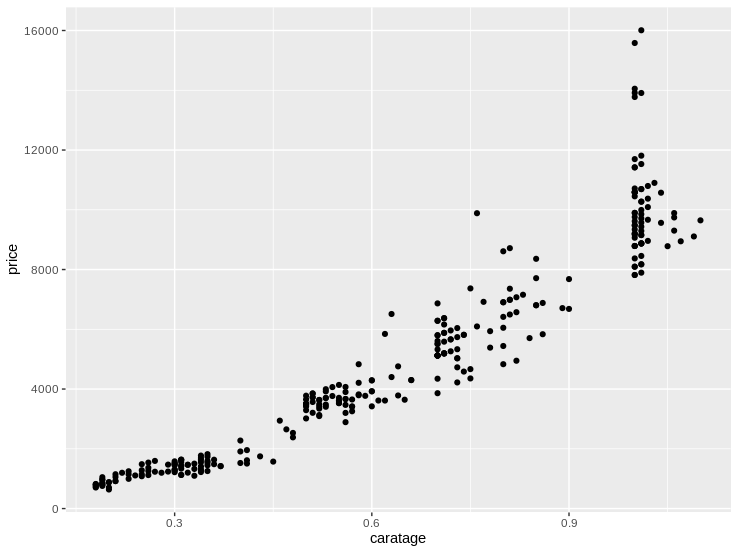
\includegraphics[width=\linewidth]{report/images/question-1/price.png}
    \caption{\texttt{price} vs \texttt{caratage}}
  \end{subfigure}
  \begin{subfigure}[b]{0.4\linewidth}
    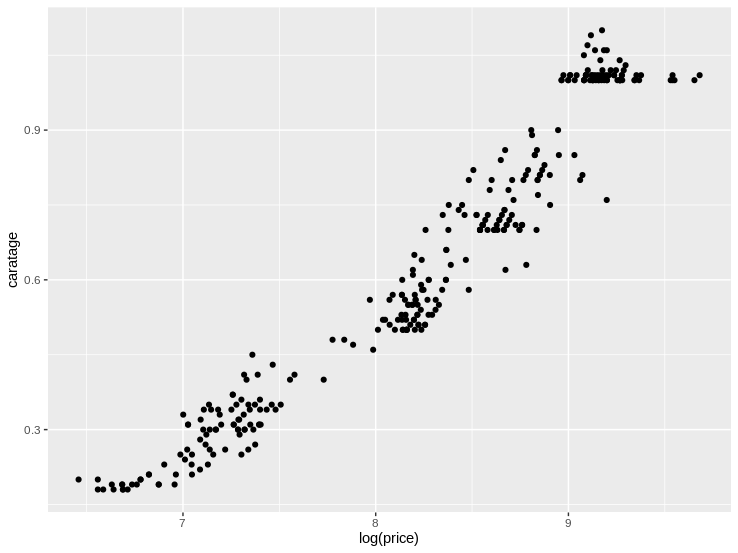
\includegraphics[width=\linewidth]{report/images/question-1/log(price).png}
    \caption{\texttt{log(price)} vs \texttt{caratage}}
  \end{subfigure}
  \caption{Gráficas para \texttt{price} y \texttt{caratage}}
  \label{fig:coffee}
\end{figure}

%%%%%%%%%%%%%%%%%%%%%%%%%%%%%%%%%%%%%%%%%
%   Pregunta 2
%%%%%%%%%%%%%%%%%%%%%%%%%%%%%%%%%%%%%%%%%
\subsection{Encuentra una manera adecuada de incluir, además de \texttt{caratage}, la otra información categórica disponible: \texttt{clarity}, \texttt{color} y \texttt{certificate}. Comenta el modelo que se ha ajustado, realizando un análisis básico de los residuos.}
\label{subsec:question-2}


%%%%%%%%%%%%%%%%%%%%%%%%%%%%%%%%%%%%%%%%%
%   Pregunta 3
%%%%%%%%%%%%%%%%%%%%%%%%%%%%%%%%%%%%%%%%%
\subsection{Crea dos acciones para remediar el resultado anterior}
\label{subsec:question-3}

\subsubsection{Crear una nueva variable categórica para segregar las piedras según caratage: digamos menos de 0,5 quilates small, de 0,5 a menos de 1 quilate (medium) y 1 quilate o más (large). Hacer small como categoría de referencia. Añadir esta nueva variable al modelo existente, así como un término de interacción entre esta nueva variable y caratage.}


\subsubsection{¿Es satisfactorio este modelo de regresión? ¿Se validan los supuestos estándar de la regresión lineal? ¿Son razonables las estimaciones numéricas?}

El resultado del test Durbin Watson refleja un p-value de 0.02904, lo que significa que hay independencia en los residuos.

El test Jarque Bera refleja un p.-value 2.2e-16 lo que significa que hay normalidad en los residuos.

El test Breusch-Pagan refleja un p-value de 7.149e-15 lo que significa que hay homogeneidad en las varianzas.

\subsubsection{Interpretar el parámetro de interacción med*carat. ¿Qué podemos inferir sobre el precio incremental del caratage en los 3 grupos?}

Para diamantes small, el precio se incrementa en 884.554 por cada 0.1 unidades de caratage*
Para diamantes medium, el precio se incrementa en 1251.772 por cada 0.1 unidades de caratage*
Para diamantes large, el precio se incrementa en 1238.55 por cada unidad de caratage

*Usamos 0.1 caratage como unidad de medida en vez de la 1 por que no tiene sentido hablar de como se incrementa el precio para los diamantes pequeños cada 1 caratage cuando el tamaño de los diamantes pequeños va de 0 a 0.5. Lo mismo pasa con los medianos.


\subsubsection{¿Qué es más valorado: el color o la claridad? }
El máximo valor de color es purityD y tiene un valor de 3180.57, mientras que el máximo valor de claridad es clarityIF y tiene un valor de 1751.03. Por lo tanto, tiene más valor la pureza de color.

\subsubsection{Siendo todas las demás variables igual, ¿cuál es la diferencia de precio medio entre un diamante de grado D y otro de grado (a) I (b) E? }

Un diamante de grado D tiene un valor medio de 3180.57, mientras que:
a) Un diamante de grado I tiene un valor medio de -3265.59, Por lo que el diamante de grado D vale 6446.16 más que uno I
b) Un diamante de grado E tiene un valor medio de 1932.54, por lo que un diamante de grado D vale 1248.03 que uno E.

\subsubsection{Siendo todas las demás variables igual, ¿existen diferencias de precio entre las piedras evaluadas por el GIA, el IGI y el HRD? }

Las evaluadas como GIA valen de media 15.21 más que el resto, las evaluadas IGI 397.34 menos que el resto y las HRD  3265.59 menos que el resto.

\subsubsection{Añade el cuadrado de \texttt{caratage} como una nueva variable explicatoria.}

\begin{figure}[h!]
  \centering
  \begin{subfigure}[b]{0.8\linewidth}
    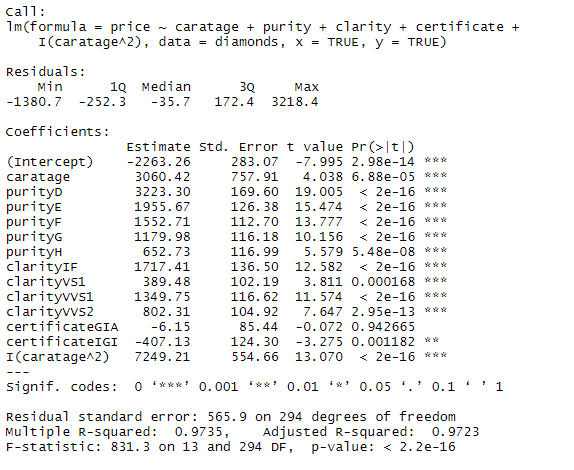
\includegraphics[width=\linewidth]{report/images/question-3/3b-summary.png}
    \caption{Summary del modelo con la nueva variable carat^2}
  \end{subfigure}
  \label{fig:coffee}
\end{figure}


%%%%%%%%%%%%%%%%%%%%%%%%%%%%%%%%%%%%%%%%%
%   Pregunta 4
%%%%%%%%%%%%%%%%%%%%%%%%%%%%%%%%%%%%%%%%%
\subsection{¿Cuál de las acciones anteriores prefieres y por qué? Justifica la respuesta en términos de interpretabilidad y validez de los supuestos.}
\label{subsec:question-4}

En términos de validez, el modelo 2, que incluye el cuadrado de la variable caratage es preferible, ya que el p-value tras aplicar a ambos modelos el método anova tiene como resultado 1.162e-08, descartando la hipótesis nula, que en este caso sería el modelo 1, que es el que incluye la variable categorica de catarage.

En términos de interpretabilidad, tiene sentido que el precio de un diamante se incremente exponencialmente con el valor de caratage (modelo 1), pero tiene menos sentido que, partiendo del modelo que ya teníamos, que incluía la variable caratage, añadiendo una variable categorica que represente umbrales de tamaño de esta variable (modelo 2) tenga algún impacto positivo en el modelo.

Por lo tanto nos quedamos con el modelo que incluye el cuadrado del caratage.

\begin{figure}[h!]
  \centering
  \begin{subfigure}[b]{0.8\linewidth}
    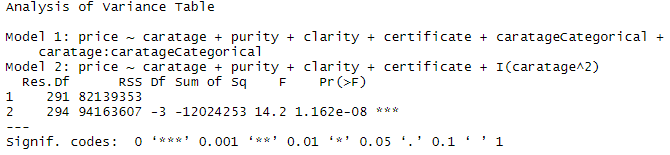
\includegraphics[width=\linewidth]{report/images/question-4/anova-exercise4.png}
    \caption{Anova model1 vs model2}
  \end{subfigure}
  \label{fig:coffee}
\end{figure}

%%%%%%%%%%%%%%%%%%%%%%%%%%%%%%%%%%%%%%%%%
\begin{thebibliography}{9}
\bibitem{bortner1969short}
    Journal of chronic diseases (Bortner, Rayman W)
    \newblock {\em A short rating scale as a potential measure of pattern A behavior}, 1969.

\end{thebibliography}

\end{document}



